\section{The Awkward Disparity between BLEU / RIBES Scores and
Human Judgments}

Automatic evaluation of machine translation (MT) quality is essential in developing high quality MT systems. 
The relatively consistent correlation of higher BLEU scores \citep{papineni2002bleu} and better human judgements in major machine translation shared tasks has led to the conventional wisdom that translations with significantly higher BLEU scores generally suggests better translation than its lower scoring counterparts \citep{bojar2014findings,WMT15,nakazawa2014overview,cettolo2014report}. 

However, automatic MT evaluation metrics have been criticized for a variety of reasons \citep{babych2004extending,callison2006re}.
\cite{callison2006re} has anecdotally presented possible failures of BLEU by showing examples of translations with the same BLEU score but of different translation quality. Through meta-evaluation\footnote{Meta-evaluation refers to the measurement of the Pearson correlation \emph{R$^2$} between an automatic evaluation metrics and human judgment scores. The meta-evaluation involves the calculation using other correlation measures such as the Spearman's rank correlation $\rho$ \citep{callison2007meta} or the Kendall's Tau $\tau$ \citep{WMT15-metric,graham-baldwin2015}} of BLEU scores and human judgements scores of the 2005 NIST MT Evaluation exercise, they have also showed high correlations of \emph{R$^2$} = 0.87 (for adequacy) and \emph{R$^2$} = 0.74 (for fluency) when an outlier rule-based machine translation system with poor BLEU score and high human score is excluded; when included the correlations drops to 0.14 for adequacy and 0.74 for fluency.


Although Callison-Burch et al. (2006) showed  poor correlation between BLEU and human scores, they had only empirically meta-evaluated a scenario where low BLEU score does not necessary result in a poor human judgement score. 

In this section, we demonstrate a real-world example of machine translation that yielded high automatic evaluation scores but failed to obtain a good score on manual evaluation in an MT shared task submission. In addition to the BLEU metric, we also evaluated our experiments results using the RIBES metric which has previously shown to have better correlations with human judgements due to its sensitivity to reordering \citep{isozaki2010automatic}. 

\subsection{BLEU}

Papineni et al. (2002) originally define BLEU \ngram{} precision \emph{p$_n$} by summing the \ngram{} matches for every hypothesis sentence $S$ in the test corpus $C$:

\begin{equation}\label{eq:bleu-precision}
{ p }_{ n }=\frac { \sum _{ S\in C }^{  }{ \sum _{ ngram\in S }^{  }{ { Count }_{ matched } } (ngram) }  }{ \sum _{ S\in C }^{  }{ \sum _{ ngram\in S }^{  }{ { Count } } (ngram) }  }
\end{equation}

BLEU is a precision based metric; to emulate recall, the brevity penalty (BP) is introduced to compensate for the possibility of high precision translations that are too short. The BP is calculated as:

\begin{equation}\label{eq:bleu-brevity}
BP = \begin{cases}
	\quad 1 \quad \qquad \text{if} \quad c \textgreater r \\
	\quad { e }^{ 1 -r/c} \quad \text{if} \quad c \le r
\end{cases}
\end{equation}

where $c$ and $r$ respectively refers to the length of the hypothesis translations and the reference translations.
The resulting system BLEU score is calculated as follows:

\begin{equation}
	\text{BLEU} = \text{BP} \times  \exp(\sum _{ n=1 }^{ N }{ { w }_{ n } \log { { p }_{ n } }  })
\end{equation}

where $n$ refers to the orders of \ngram{} considered for \emph{p$_n$} and \emph{w$_n$} refers to the weights assigned for the \ngram{} precisions; in practice, the weights are uniformly distributed.

A BLEU score can range from 0 to 1 and the closer to 1 indicates that a hypothesis translation is closer to the reference translation\footnote{Alternatively, researchers would choose to scale the BLEU score to a range between 0 to 100 to improve readability of the scores without the decimal prefix.}.

BLEU is used as the \textit{de facto} standard automatic evaluation metric for major machine translation shared tasks. And BLEU continues to show high correlations primarily for \ngram{}-based machine translation systems \citep{WMT15,nakazawa2014overview}.

However, the fallacy of BLEU-human correlations can be easily highlighted with the following example:

\newpage 
\noindent \textbf{Source}: \\
\begin{CJK*}{UTF8}{}\begin{korean}이러한 작용을 발휘하기 위해서는, \underline{각각} 0.005% 이상 함유하는 것이 바람직하다. \end{korean}\end{CJK*}
\\ \\
\noindent \textbf{Hypothesis}:  \\
\begin{CJK*}{UTF8}{min}このような 作用 を 発揮 する ため に は 、 \underline{夫 々} 0.005 % 以上 含有 する こと が 好ましい 。\end{CJK*}
\\ \\
\noindent \textbf{Baseline}:  \\
\begin{CJK*}{UTF8}{min}このような 作用 を 発揮 する ため に は 、 \underline{それぞれ} 0.005 % 以上 含有 する こと が 好ましい 。\end{CJK*}
\\ \\
\noindent \textbf{Reference}: \\
\begin{CJK*}{UTF8}{min}このような 作用 を 発揮 さ せる ため に は 、 \underline{夫 々 } 0.005 % 以上 含有 さ せる こと が 好ましい 。\end{CJK*}
\\ \\
\textbf{Source/Reference English Gloss}: \\
``So as to achieve the reaction, it is preferable that it contains more 0.005\% of \underline{each} [chemical]''
\vspace{5mm}

The unigram, bigram, trigrams and fourgrams (\emph{p$_1$}, \emph{p$_2$}, \emph{p$_3$}, \emph{p$_4$}) precision of the hypothesis translation are 90.0, 78.9, 66.7 and 52.9 respectively. The \emph{p$_n$} score for the hypothesis sentence precision score for the reference is 70.75. When considering the brevity penalty of 0.905, the overall BLEU is 64.03. Comparatively, the \ngram{} precisions for the baseline translations are \emph{p$_1$}=84.2, \emph{p$_2$}=66.7, \emph{p$_3$}=47.1 and \emph{p$_4$}=25.0 and the overall BLEU is 43.29 with a BP of 0.854. In this respect, one would consider the baseline translation inferior to the hypothesis with a \textgreater10 BLEU difference. However, there is only a subtle difference between the hypothesis and the baseline translation (\begin{CJK*}{UTF8}{min}それぞれ  vs 夫 々\end{CJK*}, which both has the same meaning).

	This is an actual example from the 2\textsuperscript{nd} Workshop on Asian Translation (WAT 2015) MT shared task evaluation, and five crowd-sourced evaluators consider the baseline translation a better translation. For this particular example, the human evaluators preferred the natural translation from Korean \begin{CJK*}{UTF8}{}\begin{korean}각각\end{korean}\end{CJK*} \emph{gaggag} to Japanese \begin{CJK*}{UTF8}{min}それぞれ\end{CJK*} \emph{sorezore} instead of the patent document usage of \begin{CJK*}{UTF8}{min}夫々\end{CJK*} \emph{sorezore}, both \begin{CJK*}{UTF8}{min}それぞれ\end{CJK*} and \begin{CJK*}{UTF8}{min}夫々\end{CJK*} can be loosely translated as '\emph{respectively}' or '\emph{(for) each}' in English.

The big difference in BLEU for a single lexical difference in translation is due to the geometric averaged scores for the individual \ngram{} precisions. It assumes the independence of \ngram{} precisions and accentuates the precision disparity by involving the single lexical difference in all possible \ngram{}s that capture the particular position in the sentence. This is clearly indicated by the growing precision difference in the higher order $n$-grams.

\subsection{RIBES}

Another failure of BLEU is the lack of explicit consideration for reordering. Callison-Burch et al. (2006) highlighted that since BLEU only takes reordering into account by rewarding the higher \ngram{} orders, freely permuted unigrams and bigrams matches are able to sustain a high BLEU score with little penalty caused by tri/fourgram mismatches. To overcome reordering, the RIBES score was introduced by adding a rank correlation coefficient\footnote{normalized Kendall $\tau$ of all \ngram{} pairs between the hypothesis and reference translations} prior to unigram matches without the need for higher order \ngram{} matches \citep{isozaki2010automatic}.

To account for word ordering, the RIBES metric first determines the word rank correlation of the word alignments by computing the Kendall's $\tau$ coefficient. Given the reference and a hypothesis translation:

\begin{enumerate}
  \item[]{\textbf{Reference}:  \textit{Alice kisses Bob yesterday}}
  \item[]{\textbf{Hypothesis}: \textit{Bob kisses Alice yesterday}}
\end{enumerate}


The first word `Alice' in the reference shifted to the third word in the hypothesis and the third word `Bob' becomes the first. The second and fourth word remains intact. From the original [0, 1, 2, 3] word order of the reference, we get the word order list [2, 1, 0, 3] in the hypothesis; where 0 = `\textit{Alice}', 1 = `\textit{kisses}', 2 = `\textit{Bob}' and 3 = `\textit{yesterday}'. 

Given the [2, 1, 0, 3] word order list of the hypothesis, we extract all possible pair of words: [(2, 1), (2, 0), (2, 3), (1, 0), (1, 3), (0, 3)]

The number of all pairs of words can be determined as $\Comb{4}{2}$ = 6. Then, we extract the pairs of words with increasing order, i.e. [(2,3), (1,3), (0,3)].

And the Kendall's $\tau$ coefficient for the word order list is compute as such:

\begin{equation}
\tau = 2 \times \frac{ no. \ of \ increasing \ pairs }{ no. \ of \ all \ pairs } -1
\end{equation}

The $\tau$ for the particular hypothesis in the example above is $\tau$ is 2 x 3/6 - 1 = 0.0. The $\tau$ coefficient ranges between [-1, 1].

To ensure that the final RIBES score ranges between 0.0 to 1.0, th e $\tau$ in the above formulation refers to the normalized Kendall $\tau$ computed as such:

\begin{equation}
\tau_{norm} = (\tau + 1)/2
\end{equation}

Simplifying BLEU's n-th order n-grams precision, the RIBES score only considers the unigram precision, $p_{1}$ using the same Equation \eqref{eq:bleu-precision} with n=1. Similarly, the RIBES brevity penalty, $BP$, follows the BLEU formulation in Equation \eqref{eq:bleu-brevity}

The final RIBES computation scales the unigram precision and brevity penalty by the Kendall's $\tau$ coefficient.

\begin{equation}
RIBES = \tau_{norm} *\ \alpha (p_{1}) *\ \beta (BP)
\end{equation}

where, $\alpha$ and $beta$ are hyperparameter used as a prior for the unigram precision and brevity penalty. They are set as $\alpha$=0.25 and $\beta$=0.10 based on the correlation with human evaluation in \citep{isozaki2010automatic}. 

Let us consider another example:
\\[0.9em]
\noindent \textbf{Source}: \\
\begin{CJK*}{UTF8}{}\begin{korean}T용융 (DSC) = 89.9℃ ; T결정화 (DSC) = 72℃ ( 5℃ / 분에서 DSC 로 측정 ) .\end{korean}\end{CJK*}
\\ \\
\noindent \textbf{Hypothesis}:  \\
\begin{CJK*}{UTF8}{min}Tmelt ( DSC ) = 7 2 ℃( 5 ℃/ 分 で DSC 測定 ( DSC ) = 89 . 9 結晶 化 度 ( T ) 。 \end{CJK*}
\\ \\
\noindent \textbf{Baseline}:  \\
\begin{CJK*}{UTF8}{min}T 溶融 ( DSC ) = 8 9 . 9 ℃; T 結晶 化 ( DSC ) = 7 2 ℃( 5 ℃/ 分 で DSC で 測定 ) 。\end{CJK*}
\\ \\
\noindent \textbf{Reference}: \\
\begin{CJK*}{UTF8}{min}Tmelt ( DSC ) = 8 9 . 9 ℃; Tcryst ( DSC ) = 7 2 ℃( 5 ℃/ 分 で DSC を 用い て 測定 ) 。\end{CJK*}
\\ \\
\textbf{Source/Reference English Gloss}: \\
Tmelt (DSC) = 8 9. 9 $^{\circ}$C; Tcryst (DSC) = 7 $^{\circ}$C (measured using DSC at 5 $^{\circ}$C / min)
\vspace{5mm}

The example above shows the marginal effectiveness of RIBES when penalizing wrongly ordered phrases in the hypothesis. The baseline translation accurately translates the meaning of the sentence with a minor partial translation of the technical variables (i.e. \emph{Tmelt} -> \emph{\begin{CJK*}{UTF8}{min}T 溶融 \end{CJK*}} and \begin{CJK*}{UTF8}{}\begin{korean}T결정화\end{korean}\end{CJK*} -> \emph{\begin{CJK*}{UTF8}{min}T 結晶 化 \end{CJK*}}. However, the hypothesis translation made serious adequacy errors when inverting the values of the technical variables but the hypothesis translation was minimally penalized in RIBES and also BLEU.

The RIBES score for the hypothesis and baseline translations are 94.04 and 86.33 respectively whereas their BLEU scores are 53.3 and 58.8. In the WAT 2015 evaluation, five evaluators unanimously voted in favor for the baseline translation. Although the RIBES score presents a wider difference between the hypothesis and baseline translation than BLEU, it is insufficient to account for the arrant error that the hypothesis translation made.

\subsection{Other Shades of BLEU / RIBES}
It is worth noting that there are other automatic MT evaluation metrics that depend on the same precision-based score with primary differences in how the \emph{Count$_{match}$(ngram)} is measured; \cite{Gimenez2007} described other linguistic features that one could match in place of surface \ngrams{}, such as lexicalized syntactic parse features, semantic entities and roles annotations, etc. As such, the modified BLEU-like metrics can present other aspects of syntactic fluency and semantic adequacy complementary to the string-based BLEU.

A different approach to improve upon the BLEU scores is to allow paraphrases or gappy variants and replace the proportion of \emph{Count$_{match}$(ngram) / \emph{Count(ngram)}} by a lexical similarity measure. \cite{banerjee2005meteor} introduced the METEOR metric that allows hypotheses' \ngram{}s to match paraphrases and stems instead of just the surface strings. \cite{lin-rouges} presented the ROUGE-S metrics that uses skip-gram matches. More recently, pre-trained regression models based on semantic textual similarity and neural network-based similarity measures trained on skip-grams are applied to replace the \ngram{} matching \citep{vela-comet,gupta-reval}.

While enriching the surface \ngram{} matching allows the automatic evaluation metric to handle variant translations, it does not resolve the ``prominent crudeness" of BLEU (Callison-Burch, 2006) involving (i) the omission of content-bearing materials not being penalized, and (ii)  the inability to calculate recall despite the brevity penalty.

\subsection{Experimental Setup}

We describe our experiment setup to evaluate Korean to Japanese patent translation using the Japan Patent Office (JPO) Patent Corpus. The JPO Patent Corpus is the official resource provided for the WAT 2015 shared task. The training dataset is made up of 1 million sentences (250k each from the chemistry, electricity, mechanical engineering and physics domains). Two development datasets\footnote{{\tt dev.txt} and {\tt devtest.txt}} and one test set each comprises 2000 sentences with 500 sentences from each of the training domains. The Korean and Japanese texts were tokenized using KoNLPy \citep{park2014konlpy} and MeCab \citep{kudo2004applying} respectively.

We used the phrase-based SMT implemented in the Moses toolkit \cite{koehn2003statistical,koehn2007moses} with the configurations as described in Chapter 2 (Section 2.4).

\subsubsection{A More Vanilla Baseline System}

\begin{table*}[!ht]
\center
    \begin{tabular}{lcc}
    \textbf{Parameters}                   & \textbf{Organizers} & \textbf{Ours}   \\ \hline
    Input document length                  & 40         & 80     \\
    Korean tokenizer                       & MeCab      & KoNLPy  \\
    Japanese tokenizer                     & Juman      & MeCab \\ \hline
	LM \ngram{} order                      & 5          & 5      \\
    Distortion limit                      & 0          & 20      \\
	Quantized \& binarized LM             & no         & yes    \\
    {\tt devtest.txt} in LM                & no         & yes    \\
    Binarized phrase tables                & no         & yes    \\
    MERT Runs               & 1         & 2    \\
    \end{tabular}
\caption{Differences between Organizer's and our Phrase-based SMT system}
\label{table-diff-between-basline-and-ours}
\end{table*}

Human evaluations were conducted as pairwise comparisons between translations from our system and the WAT organizers' phrase-based statistical MT baseline system. Table~\ref{table-diff-between-basline-and-ours} highlights the parameter differences between the organizers and our phrase-based SMT system. 

\subsubsection{Human Evaluation (Pairwise Comparison)}

The human judgment scores for the WAT evaluations were acquired using the Lancers crowdsourcing platform.
Human evaluators were randomly assigned documents from the test set.
They were shown the source document, %its reference translation, %% according to anonymous reviewer
the hypothesis translation and a baseline translation generated by the phrase-based MT system.
Five evaluators were asked to judge each document.

The crowdsourced evaluators were non-experts, thus their judgements were not necessary precise, especially for patent translations. The evaluators were asked to judge whether the hypothesis or the baseline translation was better, or they were tied. The translation that was judged better constituted a \emph{win} and the other a \emph{loss}. For each, the majority vote between the five evaluators for the hypothesis decided whether the hypothesis \emph{won}, \emph{lost} or \emph{tied} the baseline.  The final human judgment score, \emph{HUMAN}, is calculated as follows:
\begin{equation}
	\text{HUMAN} = 100 \times \frac { W-L }{ W+L+T }
\end{equation}

By definition, the \emph{HUMAN} score ranges from $-100$ to $+100$, where higher is better.

\subsection{Results}

Moses' default parameter tuning method, \mert{}, is non-deterministic, and hence it is advisable to tune the phrase-based model more than once (Clark et al. 2011). We repeated the tuning step and submitted the system translations that achieved the higher BLEU score on the development set for manual evaluation.

As a sanity check we also replicated the organizers' baseline system and submitted it for manual evaluation. We expect this system to score close to zero. We submitted a total of three sets of output to the WAT 2015 shared task, two of which underwent manual evaluation.

\begin{table}[!ht]
\center
    \begin{tabular}{lccc}
    \textbf{Systems}           & \textbf{RIBES} & \textbf{BLEU}  & \textbf{HUMAN}  \\ \hline
    Organizers'            	   &  				&   \\
    PBMT baseline         	   & 94.13				& 69.22 	& 0.0      \\ \hline
    Our  replica     		   &				& 				& \    \\
    baseline    			   & 94.29				& 70.23   & \textbf{+3.50}    \\
	Ours (\mert{} 1)              & 95.03				& 84.26 			& -      \\
	Ours (\mert{} 2)              & \textbf{95.15}				& \textbf{85.23} & -17.75 \\

    \end{tabular}
\caption{BLEU and HUMAN scores for WAT 2015}
\label{table-bleu-and-human-scores}
\end{table}

Table~\ref{table-bleu-and-human-scores} presents the BLEU scores achieved by our phrase-based MT system in contrast to the organizers' baseline phrase-based system. The difference in BLEU between the organizers' system and ours may be due to our inclusion of the second development set in building our language model and the inclusion of more training data by allowing a maximum of 80 tokens per document as compared to 40 (see Table~\ref{table-diff-between-basline-and-ours}). 

% Another major difference is the high distortion limit we have set as compared to the organizers' monotonic system, it is possible that the high distortion limit compensates for the long distance word alignments that might have been penalized by the phrasal and reordering probabilities which results in the higher RIBES and BLEU score.\footnote{In our submission {\tt Byte2String} refers to the encoding problem we encountered when tokenizing the Korean text with MeCab causing our system to read Korean bytecode instead of Unicode. But the decoder could still output Unicode since our Japanese data was successfully tokenized using MeCab, we submitted this output under the submission name {\tt Byte2String}; the {\tt Byte2String} submission is not reported in this paper. Later we rectified the encoding problem by using KoNLPy and re-ran the alignment, phrase extraction, MERT and decoding, hence the submission name, {\tt Unicode2String}, i.e. the system reported in Table~\ref{table-bleu-and-human-scores}.}

However, the puzzling fact is that our system being 15 BLEU points better than the organizers' baseline begets a terribly low human judgement score. We discuss this next.

\subsection{Segment Level Meta-Evaluation}

\begin{figure}[!htb]
    \centering
    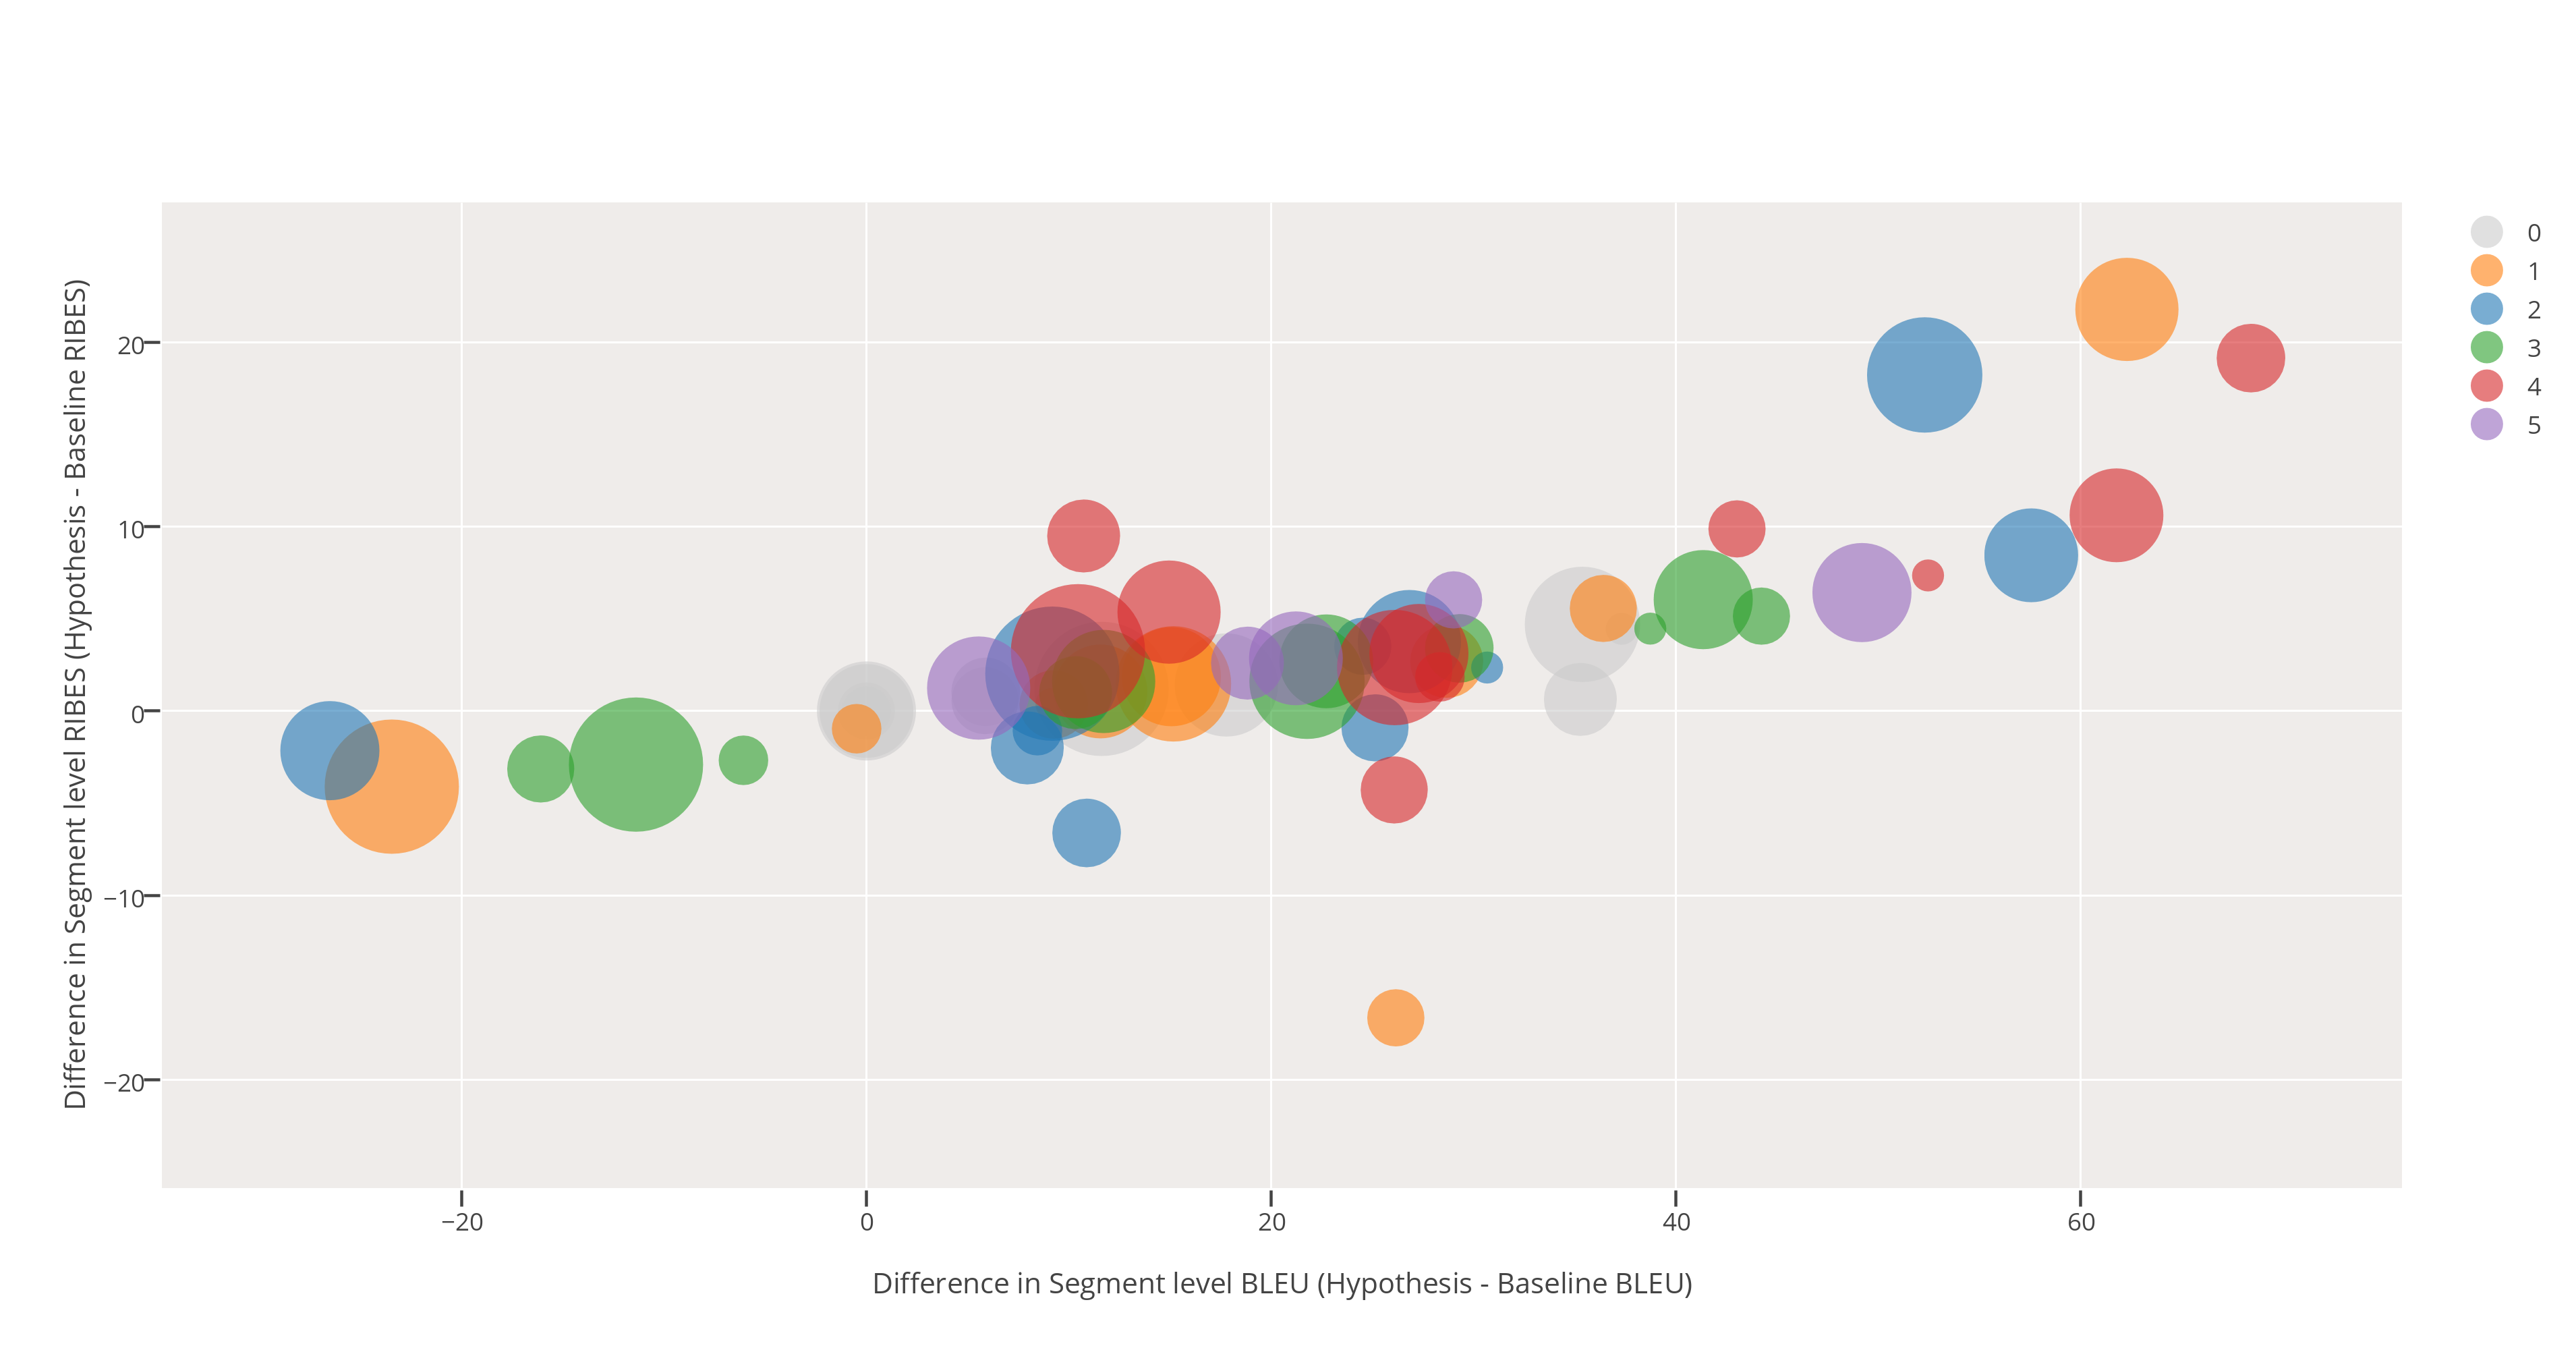
\includegraphics[width=0.8\textwidth]{diff-bleu-ribes-positive}
    \caption{Correlation between BLEU, RIBES differences and \emph{\underline{Positive}} HUMAN Judgements (HUMAN Scores of 0, +1, +2, +3, +4 and +5 represented by the colored bubbles: \emph{grey, orange, blue, green, red and purple}; larger area means more segments with the respective HUMAN Scores)}
\label{fig-cor-pos}
\end{figure}

\begin{figure}[!htb]
    \centering
    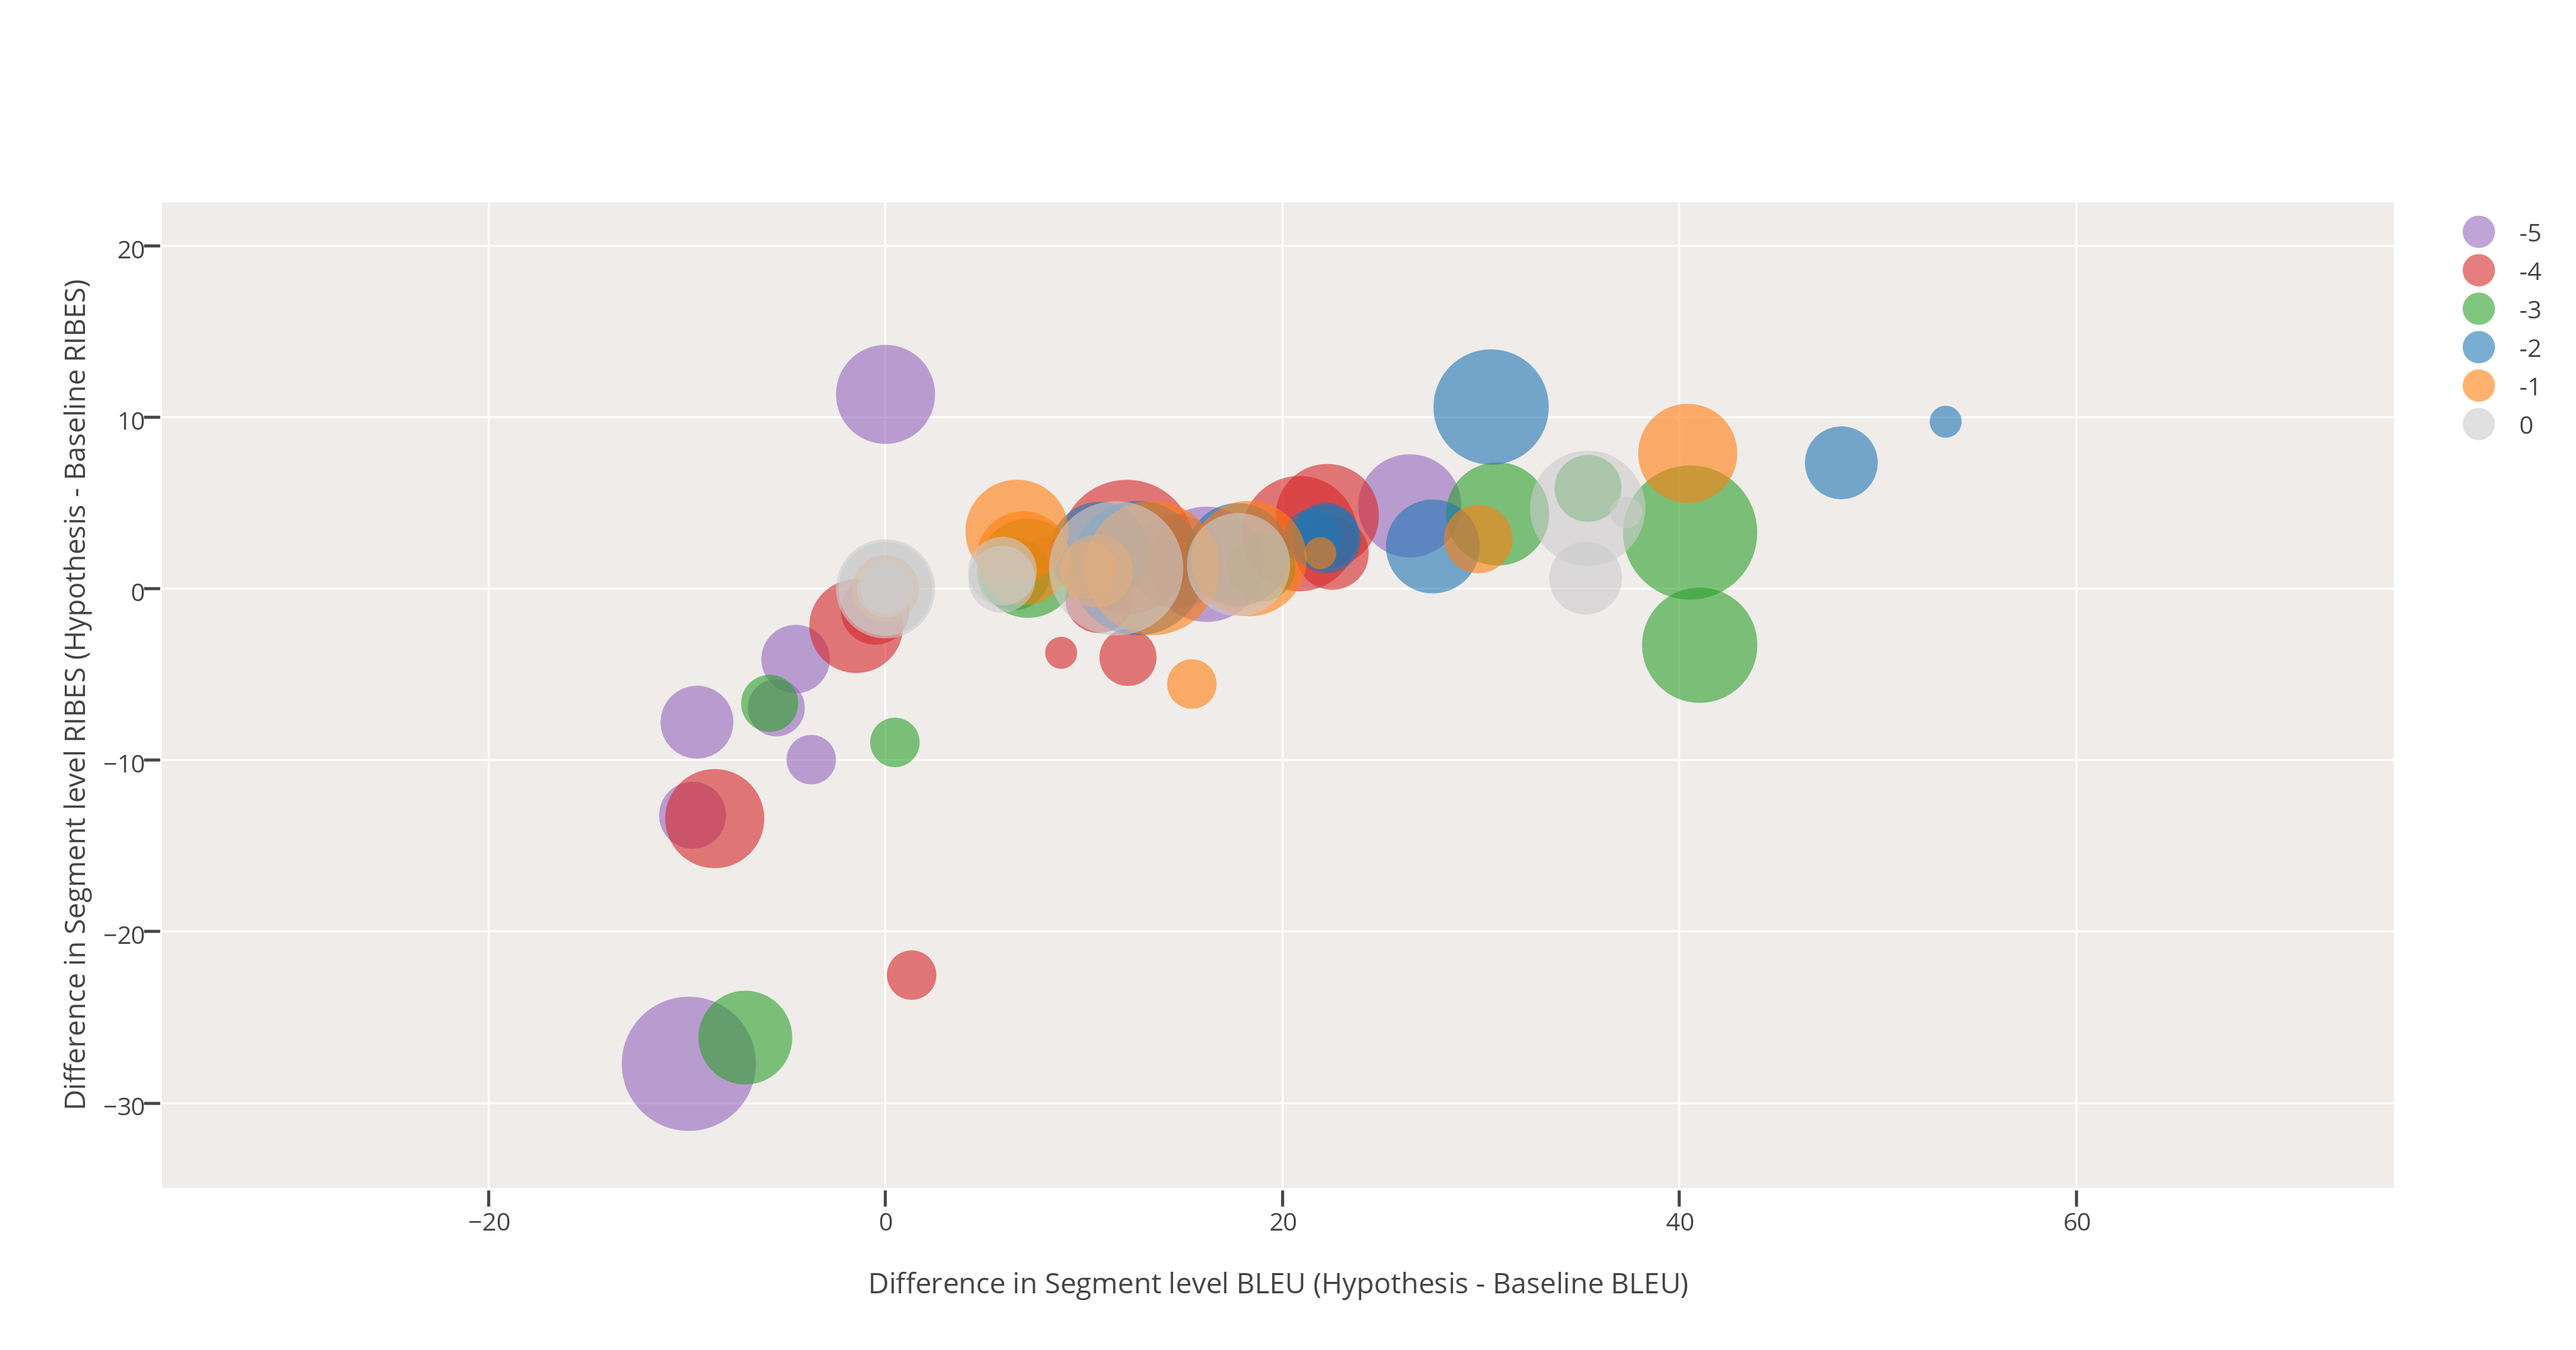
\includegraphics[width=0.8\textwidth]{diff-bleu-ribes-negative}
    \caption{Correlation between BLEU, RIBES differences and \underline{\emph{Negative}} HUMAN Judgements (HUMAN Scores of 0, -1, -2, -3, -4 and -5 represented by the colored bubbles: \emph{grey, orange, blue, green, red and purple}; larger area means more segments with the respective HUMAN Scores)}
\label{fig-cor-neg}
\end{figure}

We perform a segment level meta-evaluation by calculating the BLEU and RIBES score difference for each hypothesis-baseline translation. Figures~\ref{fig-cor-pos} and \ref{fig-cor-neg} show the correlations of the BLEU and RIBES score difference against the positive and negative human judgements score for every sentence.

Figure~\ref{fig-cor-pos} presents the considerable incongruity between our system's high BLEU improvements (>+60 BLEU) being rated marginally better than the baseline translation, indicated by the orange and blue bubbles on the top right corner. There were even translations from our system with >+40 BLEU improvements that tied with the organizer's baseline translations, indicated by the grey bubbles at around the +40 BLEU and +5 RIBES region. Except for a portion of segments that scored worse than the baseline system (lower right part of the graph where BLEU and RIBES falls below 0), the overall trend in Figure~\ref{fig-cor-pos} presents the conventional wisdom that the BLEU improvements from our systems reflects positive human judgement scores.

However, Figure~\ref{fig-cor-neg} presents the awkward disparity where many segments with BLEU improvements were rated strongly as poorer translations when compared against the baseline. Also, many segments with high BLEU improvements were tied with the baseline translations, indicated by the grey bubbles across the positive BLEU scores.

As shown in the examples in Section 2, a number of prominent factors contribute to this disparity between high BLEU / RIBES improvements and low HUMAN judgement scores:
\begin{itemize}
	\item Minor lexical differences causing a huge difference in \ngram{} precision
	\item Crowd-sourced \textit{vs}.\ expert preferences on terminology, especially for patents
	\item Minor MT evaluation metric differences not reflecting major translation inadequacy
\end{itemize}

Each of these failures contributes to an increased amount of disparity between the automatic translation metric improvements and human judgement scores.

\subsection{Summary}

In this section, we have demonstrated a real-world case where high BLEU and RIBES scores do not correlate with better human judgement. We presented several factors that might contribute to the poor correlation, and also performed a segment level meta-evaluation to identify segments where our system's high BLEU\,/\,RIBES improvements were deemed substantially worse than the baseline translations. 
We hope our results and analysis will lead to improvements in automatic translation evaluation metrics. 